
\documentclass{article}
\usepackage[utf8]{inputenc}
\usepackage[spanish]{babel}
\usepackage{graphicx}
\usepackage{listings}
 \usepackage[T1]{fontenc}
 \usepackage{subcaption}
\usepackage{float}
\usepackage{color}
\usepackage{natbib}
\usepackage{xcolor}
\usepackage{csquotes}
\usepackage{booktabs}

\usepackage {hyperref}
 \hypersetup{breaklinks=true,colorlinks=true,
        linkcolor=black,citecolor=black,urlcolor=black}

\definecolor{dkgreen}{rgb}{0,0.6,0}
\definecolor{gray}{rgb}{0.5,0.5,0.5}
\definecolor{mauve}{rgb}{0.58,0,0.82}
\definecolor{gray97}{gray}{.97}
\definecolor{gray75}{gray}{.75}
\definecolor{gray45}{gray}{.45}

\lstset{
%frame=tb,
 language=Python,
 backgroundcolor=\color{gray97},
 captionpos=b,
 keepspaces=true, 
 numbers=left,
 numbersep=5pt, 
  firstnumber=1, 
  stepnumber=1, 
  showstringspaces=false,
  tabsize=1,
% numberstyle=\small\color{migris}
 stringstyle=\color{mimalva}, 
 commentstyle=\color{miverde},
 stepnumber=1,  
 frame=single,
  escapeinside={\%*}{*)},  
  language=Python,
  aboveskip=3mm,
  belowskip=3mm,
  showstringspaces=false,
  columns=flexible,
  basicstyle={\small\ttfamily},
  %numbers=none,%esto estaba evitando que saliera la columna con los numeros en la parte del código en el documento
  %numberstyle=\tiny\color{gray},
  numberstyle=\footnotesize,
  keywordstyle=\color{blue},
  commentstyle=\color{dkgreen},
  stringstyle=\color{mauve},
  breaklines=true,
  breakatwhitespace=false,
  tabsize=3
}

\begin{document}
\title{Tarea 4 Optimización de Flujo en Redes}
\author{1985274}
\date{\today}
\maketitle 

\maketitle

En este trabajo se presenta un análisis en el que se han seleccionado 3 algoritmos generadores de grafos y a su vez se han escogido 3 implementaciones de flujo máximo. Para esto se ha utilizado el lenguaje \textbf{Python} en su versión 3.7 \cite{python}, el editor de código Spyder en su versión 3.3.1 y el editor Texmaker 5.0.2 para redactar el documento. Se utilizan además las librerías \textbf{networkX} 1.5 \cite{networkx}, \textbf{Matplotlib} \cite{matplotlib}, \textbf{Numpy}  \cite{numpy}, la librería \textbf{Panda} \cite{panda}, la librería \textbf{Scipy} \cite{scipy}, la librería \textbf{Seaborn} \cite{seaborn} para graficar, la librería \textbf{Researchcpy} \cite{researchcpy} para producir pandas Dataframe de pruebas estadísticas y \textbf{Pingouin} \cite{pingouin} para realizar el análisis de varianza de un factor (ANOVA). 

\section{Generadores}  
Se utilizaron los generadores siguientes: \textit{powerlaw cluster graph}, \textit{watts strogatz graph}, \textit{connected watts strogatz graph} y como algoritmos de flujo máximo los siguientes algoritmos: \textit{maximun flow value}, \textit{dinitz} y \textit{shortest augmenting path}.

\begin{itemize}
  \item Algoritmo \textit{powerlaw cluster graph}: o distribución en grados y agrupamiento promedio
   aproximado. Recibe 4 parámetros. Este algoritmo a cada borde aleatorio va seguido de una posibilidad haciendo una ventaja a uno de sus vecinos también.  
  \item Algoritmo \textit{watts strogatz graph}: Este es un algoritmo recibe cuatro parámetros. Primero crea un anillo sobre n nodos y luego cada nodo en el anillo es conectado con sus vecinos más cercanos. Luego se crean accesos directos 
       reemplazando algunos bordes.
  \item Algoritmo \textit{connected watts strogatz graph}: recibe 4 parámetros que son la cantidad de anillos, la cantidad de vecinos más cercano en topología anillo, la probabilidad de volver a cablear ese borde y la semilla para generar números aleatorios. 
\end{itemize}

\section{Algorítmos de flujo máximo}  

\begin{itemize}
  \item Algoritmo \textit{maximum flow value}: recibe varios parámetros entre ellos el grafo, el nodo origen para el flujo, el nodo destino. En este algoritmo el objetivo es encontrar el costo de valor máximo de un solo producto.   
  \item Algoritmo \textit{dinitz}: esta función devuelve el residual resultante después de calcular el flujo máximo.  
  \item Algoritmo \textit{shortest augmenting path} o ruta de aumento más corta. Este algoritmo tiene como idea central que cada ruta de aumento más corta se encuentra a una distancia O y cuando se aumenta el flujo a lo largo de él, al menos un borde está saturado(el flujo alcanza la capacidad). Cuando el borde se satura la distancia desde la fuente debe aumentar. 
   
\end{itemize}

A continuación un fragmento del Dataset de salida que tiene las corridas.

% Table generated by Excel2LaTeX from sheet 'Datos'
\begin{table}[htbp]
\resizebox{15cm}{!}{
\centering
\begin{tabular}{lllrrrrrrrr}
\textbf{grafo} & \textbf{generador} & \textbf{algoritmo\_flujo} & \multicolumn{1}{l}{\textbf{vertices}} & \multicolumn{1}{l}{\textbf{aristas}} & \multicolumn{1}{l}{\textbf{fuente}} & \multicolumn{1}{l}{\textbf{sumidero}} & \multicolumn{1}{l}{\textbf{media}} & \multicolumn{1}{l}{\textbf{mediana}} & \multicolumn{1}{l}{\textbf{varianza}} & \multicolumn{1}{l}{\textbf{desviacion}} \\
    vertices119aristas847 & powerlaw\_cluster\_graph & shortest\_augmenting\_path & 119   & 847   & 58    & 87    & 0.0076 & 0.00658 & 5.00E-05 & 0.00704 \\
    vertices119aristas847 & powerlaw\_cluster\_graph & dinitz & 119   & 847   & 58    & 87    & 0.02944 & 0.03124 & 1.00E-05 & 0.00364 \\
    vertices119aristas847 & powerlaw\_cluster\_graph & maximum\_flow & 119   & 847   & 58    & 87    & 0.01068 & 0.01554 & 8.00E-05 & 0.00905 \\
    vertices119aristas847 & powerlaw\_cluster\_graph & shortest\_augmenting\_path & 119   & 847   & 58    & 87    & 0.00939 & 0.01558 & 6.00E-05 & 0.00766 \\
    vertices119aristas847 & powerlaw\_cluster\_graph & dinitz & 119   & 847   & 58    & 87    & 0.03387 & 0.03129 & 1.00E-05 & 0.0032 \\
    vertices119aristas847 & powerlaw\_cluster\_graph & maximum\_flow & 119   & 847   & 58    & 87    & 0.01259 & 0.01563 & 5.00E-05 & 0.0073 \\
    vertices119aristas847 & powerlaw\_cluster\_graph & shortest\_augmenting\_path & 119   & 847   & 58    & 87    & 0.00806 & 0.00899 & 5.00E-05 & 0.00701 \\
    vertices119aristas847 & powerlaw\_cluster\_graph & dinitz & 119   & 847   & 58    & 87    & 0.03326 & 0.03484 & 0.0001 & 0.01022 \\
    vertices119aristas847 & powerlaw\_cluster\_graph & maximum\_flow & 119   & 847   & 58    & 87    & 0.0125 & 0.01562 & 4.00E-05 & 0.00625 \\
    vertices119aristas847 & powerlaw\_cluster\_graph & shortest\_augmenting\_path & 119   & 847   & 58    & 87    & 0.00626 & 0     & 6.00E-05 & 0.00767 \\
\end{tabular}%
}%    
\label{tab:addlabel}%
\caption{Fragmento del Dataset}
\end{table}%



\subsection{Código}

\lstinputlisting[language=Python, firstline=11, lastline=110]{junto.py}

\section{Análisis de varianza ANOVA}  
Luego se realizó un análisis de varianza (ANOVA) de un factor sobre estos datos, con el objetivo de comparar los tratamientos en cuanto a sus medias poblacionales. Este análisis de varianza (ANOVA) permite analizar a partir de una hipótesis si el factor tiene o no impacto en la variable tiempo \cite{fallas}.

La estimación se realizó mediante el modelo siguiente.

\begin{equation}
 y{i}{j} = \mu{1} + t{i} + \varepsilon{i}{j}  
\end{equation}

en donde:
\begin{equation}
 \mu{1}: \ \ \textup{representa la media de la población}
\end{equation}  
\begin{equation}
 t{i}: \ \ \textup{representa el efecto del tratamiento i }
\end{equation}   
\begin{equation}
 \varepsilon{i}{j}: \ \ \textup{representa el error con una distribución normal}
\end{equation} 

Si el pu da > que 0.05 se acepta la hipótesis  y esto quiere decir que no hay diferencias entre las medias , en caso contrario se rechaza la hipótesis y se pasa a aplicar el método  estadístico de Tukey.  

A continuación se obtuvieron las tablas con los resultados de la prueba de ANOVA que son las siguientes:

\begin{table}[H]
\caption{{\small de Generadores}}
%\resizebox{.5\textwidth}{!}{
\begin{center}		
	\centering
		\begin{tabular}{|r|r|r|r|r|r|r|}		
			\hline
			\textbf{Source} & \textbf{SS} & \textbf{DF} & \textbf{MS}& \textbf{F}& \textbf{p value} & \textbf{np2}\\
			
			\hline
			 Generador & 0.653 & 2 &0.326 & 0.252 &0.777 & 0 \\
			 \textit{within}    & 2327& 1797 & 1.295 & - & - & - \\			 			 
			\hline
		\end{tabular}
		\label{cual}
	%\caption{Tabla de valores capturados}
	\label{tab:una-tablita}
\end{center}	
\end{table}


\begin{table}[H]
\caption{{\small de Algoritmos de Flujo}}
\begin{center}		
	\centering
		\begin{tabular}{|r|r|r|r|r|r|r|}		
			\hline
			\textbf{Source} & \textbf{SS} & \textbf{DF} & \textbf{MS}& \textbf{F}& \textbf{p value} & \textbf{np2}\\
			
			\hline
			 Algoritmo flujo & 553.471 & 2 &276.735 & 280.187 &1.21e-106 & 0.238 \\
			 \textit{within}    & 1774& 1797 & 0.988 & - & - & - \\			 			 
			\hline
		\end{tabular}
		\label{cual}
	%\caption{Tabla de valores capturados}
	\label{tab:una-tablita}
\end{center}	
\end{table}

\begin{table}[H]
\caption{{\small de Vértices}}
\begin{center}		
	\centering
		\begin{tabular}{|r|r|r|r|r|r|r|}		
			\hline
			\textbf{Source} & \textbf{SS} & \textbf{DF} & \textbf{MS}& \textbf{F}& \textbf{p value} & \textbf{np2}\\
			
			\hline
			 Vértices & 1211.972 & 3 & 403.991 & 649.938 & 5.13e-286 & 0.521 \\
			 \textit{within}    & 1116.634& 1796 & 0.622 & - & - & - \\			 			 
			\hline
		\end{tabular}
		\label{cual}
	%\caption{Tabla de valores capturados}
	\label{tab:una-tablita}
\end{center}	
\end{table}

\begin{table}[H]
\caption{{\small de Aristas}}
\begin{center}		
	\centering
		\begin{tabular}{|r|r|r|r|r|r|r|}		
			\hline
			\textbf{Source} & \textbf{SS} & \textbf{DF} & \textbf{MS}& \textbf{F}& \textbf{p value} & \textbf{np2}\\
			
			\hline
			 Aristas & 1214.348 & 43 & 28.241 & 44.516 & 3.27e-246 & 0.522 \\
			 \textit{within}    & 1113.988& 1756 & 0.634 & - & - & - \\			 			 
			\hline
		\end{tabular}
		\label{cual}
	%\caption{Tabla de valores capturados}
	\label{tab:una-tablita}
\end{center}	
\end{table}


\section{Prueba estadística}

En esta sección se presentan los resultados de la prueba estadística \textit{Tukey} o Método de Tukey (\textit{Honestly significant difference}). Este método se utiliza luego de aplicar el ANOVA y está basada en una prueba de rango estudiantil. Una prueba de ANOVA arroja si los resultados son significativos en general, pero no aclara dónde se encuentran esas diferencias. Se emplean métodos como Tukey para averiguar qué medios de grupos específicos son diferentes, o sea para crear intervalos de confianza para todas las diferencias en parejas entre las medias de los niveles de los factores y además controla la tasa de error por familia en un nivel especificado \cite{tukey}. %La figura de la página 6 \pageref{lastPage}} 
 

En esta prueba se construyen intervalos de confianza para todas las posibles comparaciones por parejas que sigue la forma:  

\begin{equation}
 \bar{(y_{1}} - \mu_{1}), \bar{(y_{2}} - \mu_{2}),... \bar{(y_{I}} - \mu_{I}) 
\end{equation}

Este método de\textit{Tukey} resuelve el contraste:
\begin{equation}
 H_{0}: \mu_{i}= \mu_{j} \ \ \textup{ vs }   H_{1}: \mu_{i} \neq \mu_{j} 
\end{equation}
\begin{equation}
 H_{0}: \ \ \textup{Hipótesis a demostrar}
\end{equation} 
\begin{equation}
 H_{1}: \ \ \textup{Hipótesis  alternativa}
\end{equation} 

Este contraste es la hipótesis que se demostrará si es verdadera o no.

A continuación se presentan los resultados del método de \textit{Tukey}.

\begin{figure}[H] 
    \centering
              \includegraphics[width=\textwidth]{images/boxplotalgoritmoflujo.eps}
\caption{Diagrama de caja de algoritmo de flujo y la mediana}
\label{fig:seq1}
\end{figure}   

\begin{figure}[H]
    \centering
        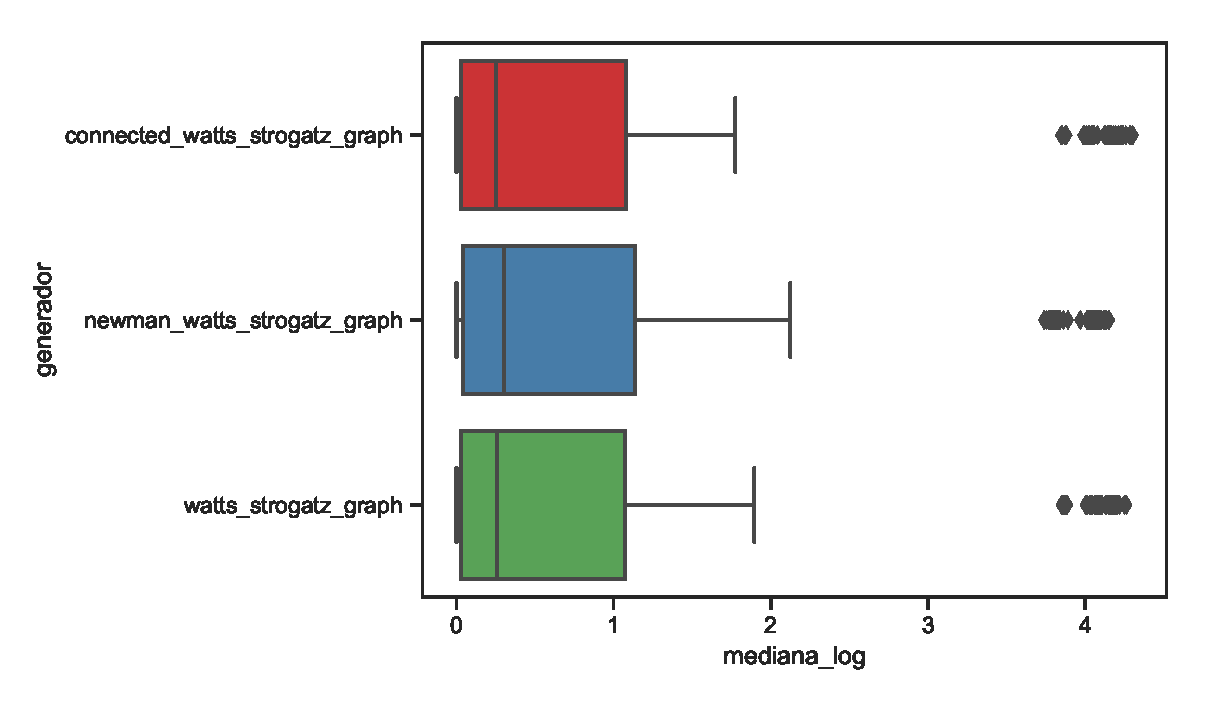
\includegraphics[width=\textwidth]{images/boxplotgenerador.eps}
        
\caption{Diagrama de caja de generadores y la mediana}
\label{fig:seq1}
\end{figure}

\begin{figure}[H] 
    \centering
        \includegraphics[width=\textwidth]{images/boxplotvertices.eps}
\caption{Diagrama de caja de vértices y la mediana}
\label{fig:seq1}
\end{figure}

A continuación las gráficas de bigote del método \textit{Tukey}.

\begin{figure}[H] 
    \centering
        \includegraphics[width=\textwidth]{images/simultaneoustukeygenerador.eps}
\caption{Gráfica de generadores y el tiempo}
\label{fig:seq1}
\end{figure} 

\begin{figure}[H] 
    \centering
        \includegraphics[width=\textwidth]{images/simultaneoustukeyalgoritmoflujo.eps}
\caption{Gráfica de algoritmos de flujo y el tiempo}
\label{fig:seq1}
\end{figure} 

\begin{figure}[H] 
    \centering
        \includegraphics[width=\textwidth]{images/simultaneoustukeyvertices.eps}
\caption{Gráfica de vértices y el tiempo}
\label{fig:seq1}
\end{figure} 

A continuación le sigue el código para aplicar la prueba de ANOVA y luego la prueba estadística de \textit{Tukey}. La variable $tukey$ almacena los resultados de la prueba Tukey. 

\subsection{Código}

\lstinputlisting[language=Python, firstline=8, lastline=60]{GSNDR1.py}

\section{Conclusión}

Se puede concluir luego del análisis del comportamiento de los datos reflejados en las tablas y en las gráficas del método estadístico \textit{Tukey} que de los factores que son los Generadores, la cantidad de nodos, la cantidad de aristas y el algoritmo de flujo máximo, el factor que más influye en la variable dependiente (el tiempo) es el factor Generador, luego le sigue el factor cantidad de nodos, y luego otro factor que influye es el algoritmo de flujo máximo y por tanto se puede llega a la conclusión de que sí inlfuyen en el tiempo.

\bibliography{ref}
\bibliographystyle{plain}

\end{document}